\section{Legge delle maglie}
La prima parte dell'esperienza consiste nel verificare la legge di Kirchoff delle maglie per un semplice partitore di tensione con due resistenze $R_1$ e $R_2$. Prima di effettuare le misure si è calcolato il valore teorico della corrente $I$ del circuito, della tensione $V_1$ ai capi di $R_1$ e della tensione $V_2$ ai capi di $R_2$. Poi si è misurato il valore dei voltaggi utilizzando un multimetro VC9205N per verificare che tali risultati fossero consistenti con l'analisi teorica. Si è usato il multimetro come un voltmetro, mettendolo quindi in parallelo con la resistenza. 

\begin{figure}
    \centering
    \begin{circuitikz}[american, voltage shift=0.5]
    \draw
    (0,0) to [voltage source,V=$V_g$,invert] (0,3)
    to [R,l=$R_1$,v=$V_{R_1}$] (3,3)
    to [R,l=$R_2$,v=$V_{R_2}$] (3,0) --(0,0);
    \draw
    (3,3) to [short] (5,3)
    to [R,R=$R_V$](5,0)--(3,0);
    \draw
    (5,3) to [short](7,3)
    to [rmeterwa,t=V](7,0)--(5,0);
    \end{circuitikz}
    \caption{Caption}
    \label{fig:enter-label}
\end{figure}


Si è ripetuto la stessa esperienza due volte, utilizzando valori diversi per le resistenze. 

Nella prima esperienza si sono usate $R_1 = 1000 \  \Omega \ (5\%) $ $R_2 = 5600 \  \Omega \ (5\%) $ $\\$ 
Si sono poi misurati i seguenti valori con il multimetro:
$\\ \\  V_0 = (5.03 \pm 0.06) \ V \\ \\ $ $V_1 = (0.79 \pm 0.07) \ V \\ \\  $ $V_2 = (4.25 \pm 0.05) \ V \\ \\ $ 
Come si vede, il valore $V_1 + V_2$ ricade nell'intervallo misurato di $V_0$


Nella seconda esperienza si sono usate $R_1 = 1 \ M   \Omega \ (5\%) $ $R_2 = 560 \ k  \Omega \ (5\%) $

Si sono poi misurati i seguenti valori con il multimetro:
$\\ \\ V_0 = (5.02 \pm 0.06) \ V \\ \\ $ $V_1 = (3.10 \pm 0.05) \ V \\ \\  $ $V_2 = (1.76 \pm 0.01) \ V \\ \\ $ 

Stavolta, se sommiamo $V_1$ e $V_2$, non ricadiamo nell'intervallo di $V_0$. Questo perchè dobbiamo considerare l'impedenza interna del multimetro, del valore nominale di $10 \ M \Omega$. Le resistenze usate rappresentano infatti una frazione considerevole di tale resistenza interna e  dobbiamo quindi modificare la nostra analisi teorica.
Quando si pone il multimetro in parallelo ad una resistenza $R_i$ dobbiamo considerare un circuito equivalente con $R^i_{eq} = \frac{R_iR_{int}}{R_i + R_{int}}$
Con la nuova analisi circuitale, si giunge al partitore equivalente con $V^1_{eq} = \frac{R_1R_{int}}{R_1 + R_{int}}V_0 =3.09  \ V $ ,  $V^2_{eq} = \frac{R_iR_{int}}{R_i + R_{int}}V_0= 1.73 \ V  $ $\\$ che, come si vede, risultano in perfetto accordo con i valori misurati e riportati precedentemente. Abbiamo deciso di procedere usando il valore nominale "esatto" di $10 \ M \Omega$ per l'impedenza interna poichè, facendo l'analisi al contrario e usando i dati per ottenere una stima di $R_{int}$, si otteneva un errore superiore al $100 \% $. Ciò è dovuto al fatto che nella formula per $R_{int}$ : $$\frac{R_1 R_2}{R_1(\frac{V_0}{V_1})-R_2}$$ il denominatore è vicino allo zero (uguale a zero per un voltmetro ideale) e di consegeunza si ottiene un errore enorme; infatti nel calcolo dell'incertezza facendo le dovute derivate tale denominatore risulterebbe elevato al quadrato. 
Si riporta comunque il risultato ottenuto ma non usato nelle analisi: $R_{int} = (10.5  \pm 12.1 ) M \Omega$

\section{Voltmetro a monte}

Si è poi ripreso il circuito con $R_1 = 1 \ M   \Omega \ (5\%) $ $R_2 = 560 \ k  \Omega \ (5\%) $ $\\$ e si è misurato $R_2$ con il metodo del voltmetro a valle e amperometro a monte, come indicato nel circuito. 

Per tale esperienza si è misurata la tensione ai capi di $R_2$ con il voltmetro e la corrente a valle del circuito con l'amperometro (multimetro TS-1010) per diversi voltaggi di ingresso $V_0$. Si è deciso di far variare $V_0$ tra $0 \ V$ e $20 \ V$ con un passo di $2.5 \ V$. Si è poi fatta l'analisi dati con python, fittando i dati con la curva teorica. Di seguito riportiamo lo schema del circuito e il grafico dei valori misurati.



\begin{figure}
    \centering
    \begin{circuitikz}[american, voltage shift=0.5]
    \draw
    (0,0) to [voltage source,V=$V_g$,invert] (0,3)
    to[rmeterwa,t=A](2,3)
    to [R,l=$R_1+R_A\approx R_1$] (4,3)
    to [R,l=$R_2$](4,0)--(0,0);
    \draw
    (4,3) to [short](6,3)
    to [R,l=$R_V$] (6,0)--(4,0);
    \draw
    (6,3) to [short](8,3)
    to[rmeterwa,t=$V$](8,0)--(6,0);
    \end{circuitikz}
    \caption{Caption}
    \label{fig:enter-label}
\end{figure}


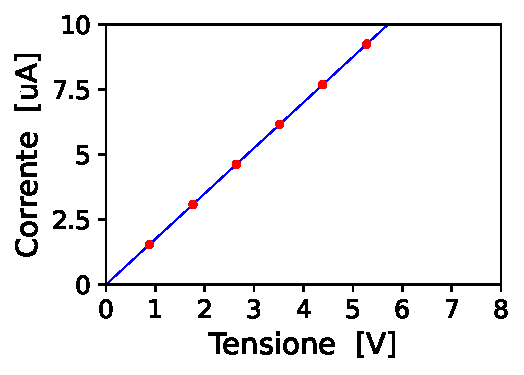
\includegraphics[scale = 1.1]{I_V_Voltmetro_Monte.pdf}


Risulta sperimentalmente $R_m = (531.1 \pm 0.7) k \Omega \\ ; $
tuttavia, questa misura rappresenta il parallelo tra $R_2$ e $R_V$. Svolgendo i calcoli, risulta $R_2 = (560.9 \pm 0.8) k \Omega$, in ottimo accordo col valore nominale. 

\section{Voltmetro a valle}

Per l'ultima parte dell'esperienza si è usato lo stesso circuito per misurare il valore di $R_2$, stavolta con la tecnica del voltmetro a monte e amperometro a valle, come indicato nel circuito in figura. Per le misure di voltaggio e tensione si sono usati gli stessi multimetri sopra citati.  Si è deciso di far variare $V_0$ tra $0 \ V$ e $20 \ V$ con un passo di $2.5 \ V$. Si è poi fatta l'analisi dati con python, fittando i dati con la curva teorica. Con i dati presi, siamo anche in grado di fornire una stima per la resistenza interna dell'amperometro. Di seguito riportiamo lo schema del circuito e il grafico dei valori misurati.


\begin{figure}
    \centering
    \begin{circuitikz}[american, voltage shift=0.5]
    \draw
    (0,0) to [voltage source,V=$V_g$,invert] (0,3)
    to [R,l=$R_1$](3,3)
    to[rmeterwa,t=$V$](3,0)--(0,0);
    \draw
    (3,3) to[short] (5,3)
    to [R,l=$R_V$](5,0)--(3,0);
    \draw
    (5,3) to [short](7,3)
    to [R,l=$R_A+R_2$](7,1.5)
    to [rmeterwa,t=A](7,0)--(5,0);
    \end{circuitikz}
    \caption{Caption}
    \label{fig:enter-label}
\end{figure}



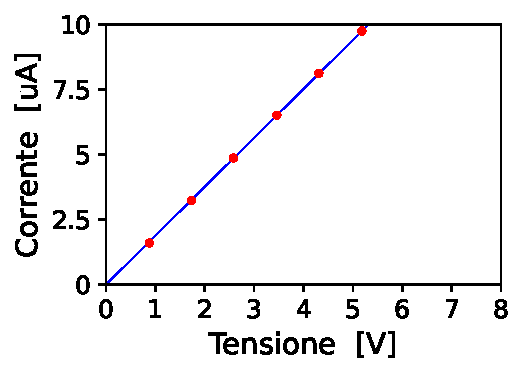
\includegraphics[scale = 1.1]{I_V_Voltmetro_Valle.pdf}

Risulta sperimentalmente $R_m = (570.4 \pm 0.2) k \Omega ; \\  $
tuttavia, questa misura rappresenta la serie tra $R_2$ e $R_A$. Possiamo anche usare il valore precedentemente ottenuto di $R_2$ per stimare $R_A$. Svolgendo i calcoli si ottiene $R_A = (9.5 \pm 10.1)k \Omega$.
